In this section, we will give a more detailed description of previous works
we directly build on and other prerequisites.

\subsection{Basic definitions}
For regression, we define the smooth $\ell_1$-loss as
\begin{equation}
\ell_1^*(x) =
\begin{cases}
0.5x^2 &\text{if |x| < 1} \\
|x| - 0.5 &\text{otherwise,}
\end{cases}
\end{equation}
which provides a certain robustness to outliers and will be used
frequently in the following chapters.
For classification we define the cross-entropy loss as
\begin{equation}
\ell_{cls} =
\end{equation}

\subsection{Optical flow and scene flow}
Let $I_1,I_2 : P \to \mathbb{R}^3$ be two temporally consecutive frames in a
sequence of images.
The optical flow
$\mathbf{w} = (u, v)^T$ from $I_1$ to $I_2$
maps pixel coordinates in the first frame $I_1$ to pixel coordinates of the
visually corresponding pixel in the second frame $I_2$,
and can be interpreted as the apparent movement of brigthness patterns between the two frames.
Optical flow can be regarded as two-dimensional motion estimation.

Scene flow is the generalization of optical flow to 3-dimensional space and
requires estimating depth for each pixel. Generally, stereo input is used for scene flow
to estimate disparity-based depth, however monocular depth estimation with deep networks is becoming
popular \cite{DeeperDepth}.

\subsection{Convolutional neural networks for dense motion estimation}
Deep convolutional neural network (CNN) architectures
\cite{ImageNetCNN, VGGNet, ResNet}
became widely popular through numerous successes in classification and recognition tasks.
The general structure of a CNN consists of a convolutional encoder, which
learns a spatially compressed, wide (in the number of channels) representation of the input image,
and a fully connected prediction network on top of the encoder.

The compressed representations learned by CNNs of these categories do not, however, allow
for prediction of high-resolution output, as spatial detail is lost through sequential applications
of pooling or strides.
Thus, networks for dense prediction introduce a convolutional decoder on top of the representation encoder,
performing upsampling of the compressed features and resulting in a encoder-decoder pyramid.
The most popular deep networks of this kind for end-to-end optical flow prediction
are variants of the FlowNet family \cite{FlowNet, FlowNet2},
which was recently extended to scene flow estimation \cite{SceneFlowDataset}.
Table \ref{} shows the classical FlowNetS architecture for optical fow prediction.
Note that the network itself is a rather generic autoencoder and is specialized for optical flow only through being trained
with supervision from dense optical flow ground truth.
Potentially, the same network could also be used for semantic segmentation if
the number of output channels was adapted from two to the number of classes. % TODO verify
Still, FlowNetS demonstrates that a generic deep encoder-decoder CNN can learn to perform image matching arguably well,
given just two consecutive frames as input and a large enough receptive field at the outputs to cover the displacements.
Note that the maximum displacement that can be correctly estimated only depends on the number of 2D strides or pooling
operations in the encoder.
Recently, other encoder-decoder CNNs have been applied to optical flow as well \cite{DenseNetDenseFlow}.

\subsection{SfM-Net}
Here, we will describe the SfM-Net \cite{SfmNet} architecture in more detail and show their results
and some of the issues.

\subsection{ResNet}
\label{ssec:resnet}
ResNet \cite{ResNet} was initially introduced as a CNN for image classification, but
became popular as basic building block of many deep network architectures for a variety
of different tasks. In Table \ref{table:resnet}, we show the ResNet-50 variant
that will serve as the basic CNN backbone of our networks, and
is also used in many other region-based convolutional networks.
The initial image data is always passed through ResNet-50 as a first step to
bootstrap the complete deep network.
Figure \ref{figure:bottleneck}
shows the fundamental building block of ResNet-50.

{
%\begin{table}[h]
%\centering
\begin{longtable}{llr}
\toprule
\textbf{Layer ID} & \textbf{Layer Operations} & \textbf{Output Dimensions} \\
\midrule\midrule
 & input image & H $\times$ W $\times$ C \\
\midrule
\multicolumn{3}{c}{\textbf{ResNet-50}}\\
\midrule
C$_1$ & 7 $\times$ 7 conv, 64, stride 2 & $\tfrac{1}{2}$ H $\times$ $\tfrac{1}{2}$ W $\times$ 64 \\

& 3 $\times$ 3 max pool, stride 2 & $\tfrac{1}{4}$ H $\times$ $\tfrac{1}{4}$ W $\times$ 64 \\

C$_2$ &
$\begin{bmatrix}
1 \times 1, 64 \\
3 \times 3, 64 \\
1 \times 1, 256 \\
\end{bmatrix}_b$ $\times$ 3
& $\tfrac{1}{4}$ H $\times$ $\tfrac{1}{4}$ W $\times$ 256 \\
\midrule
C$_3$ &
$\begin{bmatrix}
1 \times 1, 128 \\
3 \times 3, 128 \\
1 \times 1, 512 \\
\end{bmatrix}_{b/2}$ $\times$ 4
& $\tfrac{1}{8}$ H $\times$ $\tfrac{1}{8}$ W $\times$ 512 \\
\midrule
C$_4$ &
$\begin{bmatrix}
1 \times 1, 256 \\
3 \times 3, 256 \\
1 \times 1, 1024 \\
\end{bmatrix}_{b/2}$ $\times$ 6
& $\tfrac{1}{16}$ H $\times$ $\tfrac{1}{16}$ W $\times$ 1024 \\
\midrule
C$_5$ &
$\begin{bmatrix}
1 \times 1, 512 \\
3 \times 3, 512 \\
1 \times 1, 2048 \\
\end{bmatrix}_{b/2}$ $\times$ 3
& $\tfrac{1}{32}$ H $\times$ $\tfrac{1}{32}$ W $\times$ 1024 \\

\bottomrule

\caption {
ResNet-50 \cite{ResNet} architecture (Figure from \cite{ResNet}).
Operations enclosed in a []$_b$ block make up a single ResNet \enquote{bottleneck}
block (see Figure \ref{figure:bottleneck}). If the block is denoted as []$_b/2$,
the first conv operation in the block has a stride of 2. Note that the stride
is only applied to the first block, but not to repeated blocks.
}
\label{table:resnet}
\end{longtable}


%\end{table}
}

\begin{figure}[t]
  \centering
  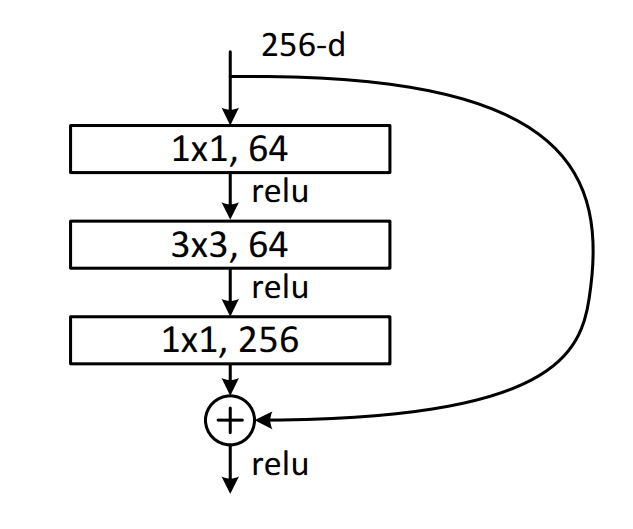
\includegraphics[width=0.3\textwidth]{figures/bottleneck}
\caption{
ResNet \cite{ResNet} \enquote{bottleneck} convolutional block introduced to reduce computational
complexity in deeper network variants, shown here with 256 input and output channels.
}
\label{figure:bottleneck}
\end{figure}

\subsection{Region-based convolutional networks}
\label{ssec:rcnn}
We now give an overview of region-based convolutional networks, which are currently by far the
most popular deep networks for object detection, and have recently also been applied to instance segmentation.

\paragraph{R-CNN}
Region-based convolutional networks (R-CNNs) \cite{RCNN} use a non-learned algorithm external to a standard encoder CNN
for computing \emph{region proposals} in the shape of 2D bounding boxes, which represent regions that may contain an object.
For each of the region proposals, the input image is cropped using the regions bounding box and the crop is
passed through a CNN, which performs classification of the object (or non-object, if the region shows background).

\paragraph{Fast R-CNN}
The original R-CNN involves computing one forward pass of the CNN for each of the region proposals,
which is costly, as there is generally a large number of proposals.
Fast R-CNN \cite{FastRCNN} significantly reduces computation by performing only a single forward pass with the whole image
as input to the CNN (compared to the sequential input of crops in the case of R-CNN).
Then, fixed size crops are taken from the compressed feature map of the image,
each corresponding to one of the proposal bounding boxes.
The crops are collected into a batch and passed into a small Fast R-CNN
\emph{head} network, which performs classification and prediction of refined boxes for all regions in one forward pass.
This technique is called \emph{RoI pooling}. % TODO explain how RoI pooling converts full image box coords to crop ranges
\todo{more details and figure}
Thus, given region proposals, the per-region computation is reduced to a single pass through the complete network,
speeding up the system by orders of magnitude. % TODO verify that

\paragraph{Faster R-CNN}
After streamlining the CNN components, Fast R-CNN is limited by the speed of the region proposal
algorithm, which has to be run prior to the network passes and makes up a large portion of the total
processing time.
The Faster R-CNN object detection system \cite{FasterRCNN} unifies the generation of region proposals and subsequent box refinement and
classification into a single deep network, leading to faster processing when compared to Fast R-CNN
and again, improved accuracy.
This unified network operates in two stages.
In the \emph{first stage}, one forward pass is performed on the \emph{backbone} network,
which is a deep feature encoder CNN with the original image as input.
Next, the \emph{backbone} output features are passed into a small, fully convolutional \emph{Region Proposal Network (RPN)} head, which
predicts objectness scores and regresses bounding boxes at each of its output positions.
At any position, bounding boxes are predicted as offsets relative to a fixed set of \emph{anchors} with different
aspect ratios.
\todo{more details and figure}
% TODO more about striding & computing the anchors?
For each anchor at a given position, the objectness score tells us how likely this anchors is to correspond to a detection.
The region proposals can then be obtained as the N highest scoring anchor boxes.

The \emph{second stage} corresponds to the original Fast R-CNN head network, performing classification
and bounding box refinement for each region proposal. % TODO verify that it isn't modified
As in Fast R-CNN, RoI pooling is used to crop one fixed size feature map for each of the region proposals.


\paragraph{Mask R-CNN}
Faster R-CNN and the earlier systems detect and classify objects at bounding box granularity.
However, it can be helpful to know class and object (instance) membership of all individual pixels,
which generally involves computing a binary mask for each object instance specifying which pixels belong
to that object. This problem is called \emph{instance segmentation}.
Mask R-CNN \cite{MaskRCNN} extends the Faster R-CNN system to instance segmentation by predicting
fixed resolution instance masks within the bounding boxes of each detected object.
This is done by simply extending the Faster R-CNN head with multiple convolutions, which
compute a pixel-precise mask for each instance.
The basic Mask R-CNN ResNet-50 architecture is shown in Table \ref{table:maskrcnn_resnet}.
\todo{RoI Align}

{
%\begin{table}[t]
%\centering
\begin{longtable}{llr}
\toprule
\textbf{Layer ID} & \textbf{Layer Operations} & \textbf{Output Dimensions} \\
\midrule\midrule
& input image & H $\times$ W $\times$ C \\
\midrule
C$_4$ & ResNet-50 \{up to C$_4$\} (Table \ref{table:resnet})  & $\tfrac{1}{16}$ H $\times$ $\tfrac{1}{16}$ W $\times$ 1024 \\
\midrule
\multicolumn{3}{c}{\textbf{Region Proposal Network (RPN)}}\\
\midrule
& From C$_4$: 1 $\times$ 1 conv, 512 & $\tfrac{1}{16}$ H $\times$ $\tfrac{1}{16}$ W $\times$ 512 \\
& 1 $\times$ 1 conv, 6 & $\tfrac{1}{16}$ H $\times$ $\tfrac{1}{16}$ W $\times$ 6 \\
& flatten & A $\times$ 6 \\
 & decode bounding boxes (Eq. \ref{eq:pred_bounding_box}) & A $\times$ 6 \\
ROI$_{\mathrm{RPN}}$ & sample bounding boxes \& scores (Listing \ref{}) & N$_{RPN}$ $\times$ 6 \\
\midrule
\multicolumn{3}{c}{\textbf{RoI Head}}\\
\midrule
& From C$_4$ with ROI$_{\mathrm{RPN}}$: RoI pooling (\ref{}) & N$_{RPN}$ $\times$ 7 $\times$ 7 $\times$ 1024 \\
R$_1$& ResNet-50 \{C$_5$ without stride\} (Table \ref{table:resnet})  & N$_{RPN}$ $\times$ 7 $\times$ 7 $\times$ 2048 \\
ave & average pool & N$_{RPN}$ $\times$ 2048 \\
boxes& From ave: fully connected, 4 & N$_{RPN}$ $\times$ 4 \\
logits& From ave: fully connected, N$_{cls}$ & N$_{RPN}$ $\times$ N$_{cls}$ \\
\midrule
\multicolumn{3}{c}{\textbf{RoI Head: Masks}}\\
\midrule
& From R$_1$: 2 $\times$ 2 deconv, 256, stride 2 & N$_{RPN}$ $\times$ 14 $\times$ 14 $\times$ 256 \\
masks & 1 $\times$ 1 conv, N$_{cls}$ & N$_{RPN}$ $\times$ 14 $\times$ 14 $\times$ N$_{cls}$ \\

\bottomrule

\caption {
Mask R-CNN \cite{MaskRCNN} ResNet-50 \cite{ResNet} architecture.
Note that this is equivalent to the Faster R-CNN architecture if the mask
head is left out.
}
\label{table:maskrcnn_resnet}
\end{longtable}
%\end{table}
}

\paragraph{Feature Pyramid Networks}
In Faster R-CNN, a single feature map is used as a source of all RoIs, independent
of the size of the bounding box of the RoI.
However, for small objects, the C$_4$ (see Table \ref{table:maskrcnn_resnet}) features
might have lost too much spatial information to properly predict the exact bounding
box and a high resolution mask. Likewise, for very big objects, the fixed size
RoI window might be too small to cover the region of the feature map containing
information for this object.
As a solution to this, the Feature Pyramid Network (FPN) \cite{FPN} enable features
of an appropriate scale to be used, depending of the size of the bounding box.
For this, a pyramid of feature maps is created on top of the ResNet \cite{ResNet}
encoder. \todo{figure and more details}
Now, during RoI pooling,
\todo{show formula}.
The Mask R-CNN ResNet-50-FPN variant is shown in Table \ref{table:maskrcnn_resnet_fpn}.

{
%\begin{table}[t]
%\centering
\begin{longtable}{llr}
\toprule
\textbf{Layer ID} & \textbf{Layer Operations} & \textbf{Output Dimensions} \\
\midrule\midrule
& input image & H $\times$ W $\times$ C \\
\midrule
C$_5$ & ResNet-50 (Table \ref{table:resnet})  & $\tfrac{1}{32}$ H $\times$ $\tfrac{1}{32}$ W $\times$ 1024 \\
\midrule
\multicolumn{3}{c}{\textbf{Feature Pyramid Network (FPN)}}\\
\midrule
P$_5$ & From C$_5$: 1 $\times$ 1 conv, 256 & $\tfrac{1}{32}$ H $\times$ $\tfrac{1}{32}$ W $\times$ 256 \\
P$_4$ & $\begin{bmatrix}\textrm{skip from C$_4$}\end{bmatrix}_p$ & $\tfrac{1}{16}$ H $\times$ $\tfrac{1}{16}$ W $\times$ 256 \\
P$_3$ & $\begin{bmatrix}\textrm{skip from C$_3$}\end{bmatrix}_p$ & $\tfrac{1}{8}$ H $\times$ $\tfrac{1}{8}$ W $\times$ 256 \\
P$_2$ & $\begin{bmatrix}\textrm{skip from C$_2$}\end{bmatrix}_p$ & $\tfrac{1}{4}$ H $\times$ $\tfrac{1}{4}$ W $\times$ 256 \\
P$_6$ & From P$_5$: 2 $\times$ 2 subsample, 256 & $\tfrac{1}{64}$ H $\times$ $\tfrac{1}{64}$ W $\times$ 256 \\
\midrule
\multicolumn{3}{c}{\textbf{Region Proposal Network (RPN)}}\\
\midrule
\multicolumn{3}{c}{$\forall i \in \{2...6\}$}\\
& From P$_i$: 1 $\times$ 1 conv, 512 & $\tfrac{1}{2^i}$ H $\times$ $\tfrac{1}{2^i}$ W $\times$ 512 \\
& 1 $\times$ 1 conv, 6 & $\tfrac{1}{2^i}$ H $\times$ $\tfrac{1}{2^i}$ W $\times$ 6 \\
RPN$_i$& flatten & A$_i$ $\times$ 6 \\
\midrule
& From \{RPN$_2$ ... RPN$_6$\}: concatenate & A $\times$ 6 \\
& decode bounding boxes (Eq. \ref{eq:pred_bounding_box}) & A $\times$ 6 \\
ROI$_{\mathrm{RPN}}$ & sample bounding boxes \& scores (Listing \ref{}) & N$_{RPN}$ $\times$ 6 \\
\midrule
\multicolumn{3}{c}{\textbf{RoI Head}}\\
\midrule
R$_2$ & From \{P$_2$ ... P$_6$\} with ROI$_{\mathrm{RPN}}$: FPN RoI crop & N$_{RPN}$ $\times$ 14 $\times$ 14 $\times$ 256 \\
& 2 $\times$ 2 max pool & N$_{RPN}$ $\times$ 7 $\times$ 7 $\times$ 256 \\
F$_1$ & $\begin{bmatrix}\textrm{fully connected}, 1024\end{bmatrix}$ $\times$ 2 & N$_{RPN}$ $\times$ 1024 \\
boxes& From F$_1$: fully connected, 4 & N$_{RPN}$ $\times$ 4 \\
logits& From F$_1$: fully connected, N$_{cls}$ & N$_{RPN}$ $\times$ N$_{cls}$ \\
\midrule
\multicolumn{3}{c}{\textbf{RoI Head: Masks}}\\
\midrule
& From R$_2$: $\begin{bmatrix}\textrm{3 $\times$ 3 conv} \end{bmatrix}$ $\times$ 4, 256 & N$_{RPN}$ $\times$ 14 $\times$ 14 $\times$ 256 \\
& 2 $\times$ 2 deconv, 256, stride 2 & N$_{RPN}$ $\times$ 28 $\times$ 28 $\times$ 256 \\
masks & 1 $\times$ 1 conv, N$_{cls}$ & N$_{RPN}$ $\times$ 28 $\times$ 28 $\times$ N$_{cls}$ \\
\bottomrule

\caption {
Mask R-CNN \cite{MaskRCNN} ResNet-50-FPN \cite{ResNet} architecture.
Operations enclosed in a []$_p$ block make up a single FPN
block (see Figure \ref{figure:fpn_block}).
}
\label{table:maskrcnn_resnet_fpn}
\end{longtable}
%\end{table}
}

\begin{figure}[t]
  \centering
  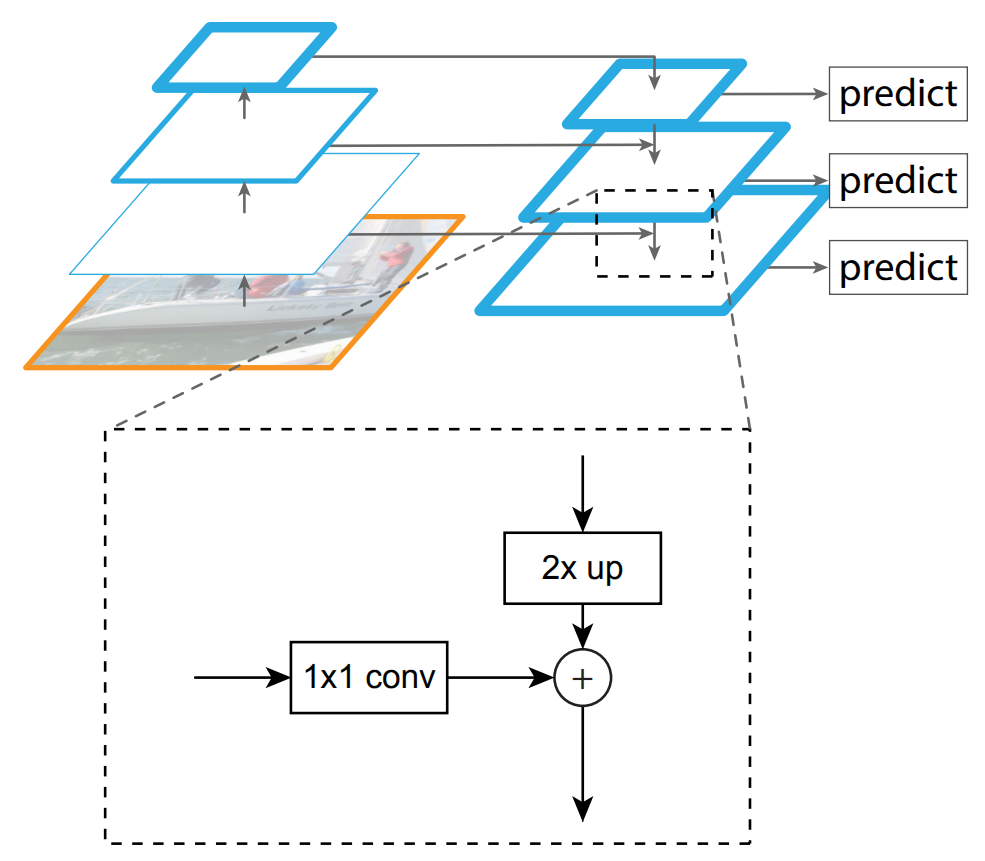
\includegraphics[width=0.3\textwidth]{figures/fpn}
\caption{
FPN block from \cite{FPN}.
Lower resolution features coming from the bottleneck are bilinearly upsampled
and added with higher resolution skip connections from the encoder.
}
\label{figure:fpn_block}
\end{figure}

\subsection{Training Mask R-CNN}
\label{ssec:rcnn_techn}
\paragraph{Bounding box regression}
All bounding boxes predicted by the RoI head or RPN are estimated as offsets
with respect to a reference bounding box. In the case of the RPN,
the reference bounding box is one of the anchors, and refined bounding boxes from the RoI head are
predicted relative to the RPN output bounding boxes.
Let $(x, y, w, h)$ be the top left coordinates, height and width of the bounding box
to be predicted. Likewise, let $(x^*, y^*, w^*, h^*)$ be the ground truth bounding
box and let $(x_r, y_r, w_r, h_r)$ be the reference bounding box.
We then define the ground truth \emph{box encoding} $b_e^*$ as
\begin{equation}
b_e^* = (b_x^*, b_y^*, b_w^*, b_h^*),
\end{equation}
where
\begin{equation*}
b_x^* = \frac{x^* - x_r}{w_r},
\end{equation*}
\begin{equation*}
b_y^* = \frac{y^* - y_r}{h_r}
\end{equation*}
\begin{equation*}
b_w^* = \log \left( \frac{w^*}{w_r} \right)
\end{equation*}
\begin{equation*}
b_h^* = \log \left( \frac{h^*}{h_r} \right),
\end{equation*}
which represents the regression target for the bounding box refinement
outputs of the network.

In the same way, we define the predicted box encoding $b_e$ as
\begin{equation}
b_e = (b_x, b_y, b_w, b_h),
\end{equation}
where
\begin{equation*}
b_x = \frac{x - x_r}{w_r},
\end{equation*}
\begin{equation*}
b_y = \frac{y - y_r}{h_r}
\end{equation*}
\begin{equation*}
b_w = \log \left( \frac{w}{w_r} \right)
\end{equation*}
\begin{equation*}
b_h = \log \left( \frac{h}{h_r} \right).
\end{equation*}

At test time, to get from a predicted box encoding $b_e$ to the predicted bounding box $b$,
we invert the definitions above,
\begin{equation}
b = (x, y, w, h),
\label{eq:pred_bounding_box}
\end{equation}
where
\begin{equation*}
x = b_x \cdot w_r + x_r,
\end{equation*}
\begin{equation*}
y = b_y \cdot b_r + y_r,
\end{equation*}
\begin{equation*}
w = \exp(b_w) \cdot w_r,
\end{equation*}
\begin{equation*}
h = \exp(b_h) \cdot h_r,
\end{equation*}
and thus obtain the bounding box as the reference bounding box adjusted by
the predicted relative offsets and scales.


\paragraph{Supervision of the RPN}
\todo{TODO}

\paragraph{Supervision of the RoI head}
\todo{TODO}
